\subsection{Simulation Platform}
\label{sec:simulation_platform}

To support efficient and reproducible evaluation of generalist manipulation policies, RoboDojo builds a configurable simulation platform based on NVIDIA Isaac Sim~\citep{NVIDIA_Isaac_Sim} and Isaac Lab~\citep{mittal2025isaaclab}. The platform comprises three main components: a configuration-driven simulation stack, a physically grounded digital asset library, and a heterogeneous parallel execution mechanism. Together, these components support diverse task construction, scalable policy evaluation, and efficient demonstration collection. Additional implementation details are provided in Appendix~\ref{appendix:Simulation_Platform}.

\subsubsection{Simulation Platform Setup}

RoboDojo uses the vectorized execution interface of Isaac Lab~\citep{mittal2025isaaclab} as the simulation backend, and builds its simulation stack on the infrastructure of MagicSim~\citep{lu2026magicsim}, inheriting its modular manager architecture, configuration-driven scene construction pipeline, and object simulation backend. Each task is instantiated from modular YAML specifications that define task assets, scene layouts, initialization distributions, randomization ranges, and success conditions. This design decouples task specification from simulator execution, allowing different tasks to share the same runtime while varying task-specific objects, scene layouts, and reset distributions, details can be found in ~\ref{appendix:simulation_platform_details}.

At reset time, RoboDojo samples task-relevant objects, object poses, articulation states, clutter layouts, lighting conditions, and background textures with deterministic seed control. This enables diverse yet reproducible scene instances for both training and evaluation. The same scene construction pipeline supports rigid, articulated, and deformable assets through a unified interface. Details of the configuration format, randomization parameters, and scene construction pipeline are provided in Appendix~\ref{appendix:simulation_platform_setup}.

\subsubsection{Physically Grounded Digital Asset Library}

RoboDojo builds a digital asset library containing rigid, articulated, and deformable objects. These assets are used as both task-relevant objects and clutter distractors across simulation tasks, enabling diverse scene instantiations while maintaining reliable physical behavior for contact-rich manipulation, inspired by ManiTwin~\citep{wang2026manitwin}. Rigid objects are collected from online repositories and reconstructed from real-world daily objects using Meshy AI\footnote{\url{https://www.meshy.ai/}}. Each asset is annotated with semantic and task-level metadata, including object categories, language descriptions, placement regions, success-checking annotations, and manipulation affordances.

Articulated and deformable assets are collected from open-source platforms, 3D scanning, and selected assets from ClothesNet~\citep{zhou2023clothesnet}. Before being used in RoboDojo tasks, these assets are standardized in terms of kinematic structure, collision geometry, material parameters, and simulation-ready representations. Details on asset processing, annotation, and physical validation are provided in Appendix~\ref{appendix:asset_library_details}.

\begin{figure}[h]
    \centering
    \begin{subfigure}[t]{0.5\textwidth}
        \centering
        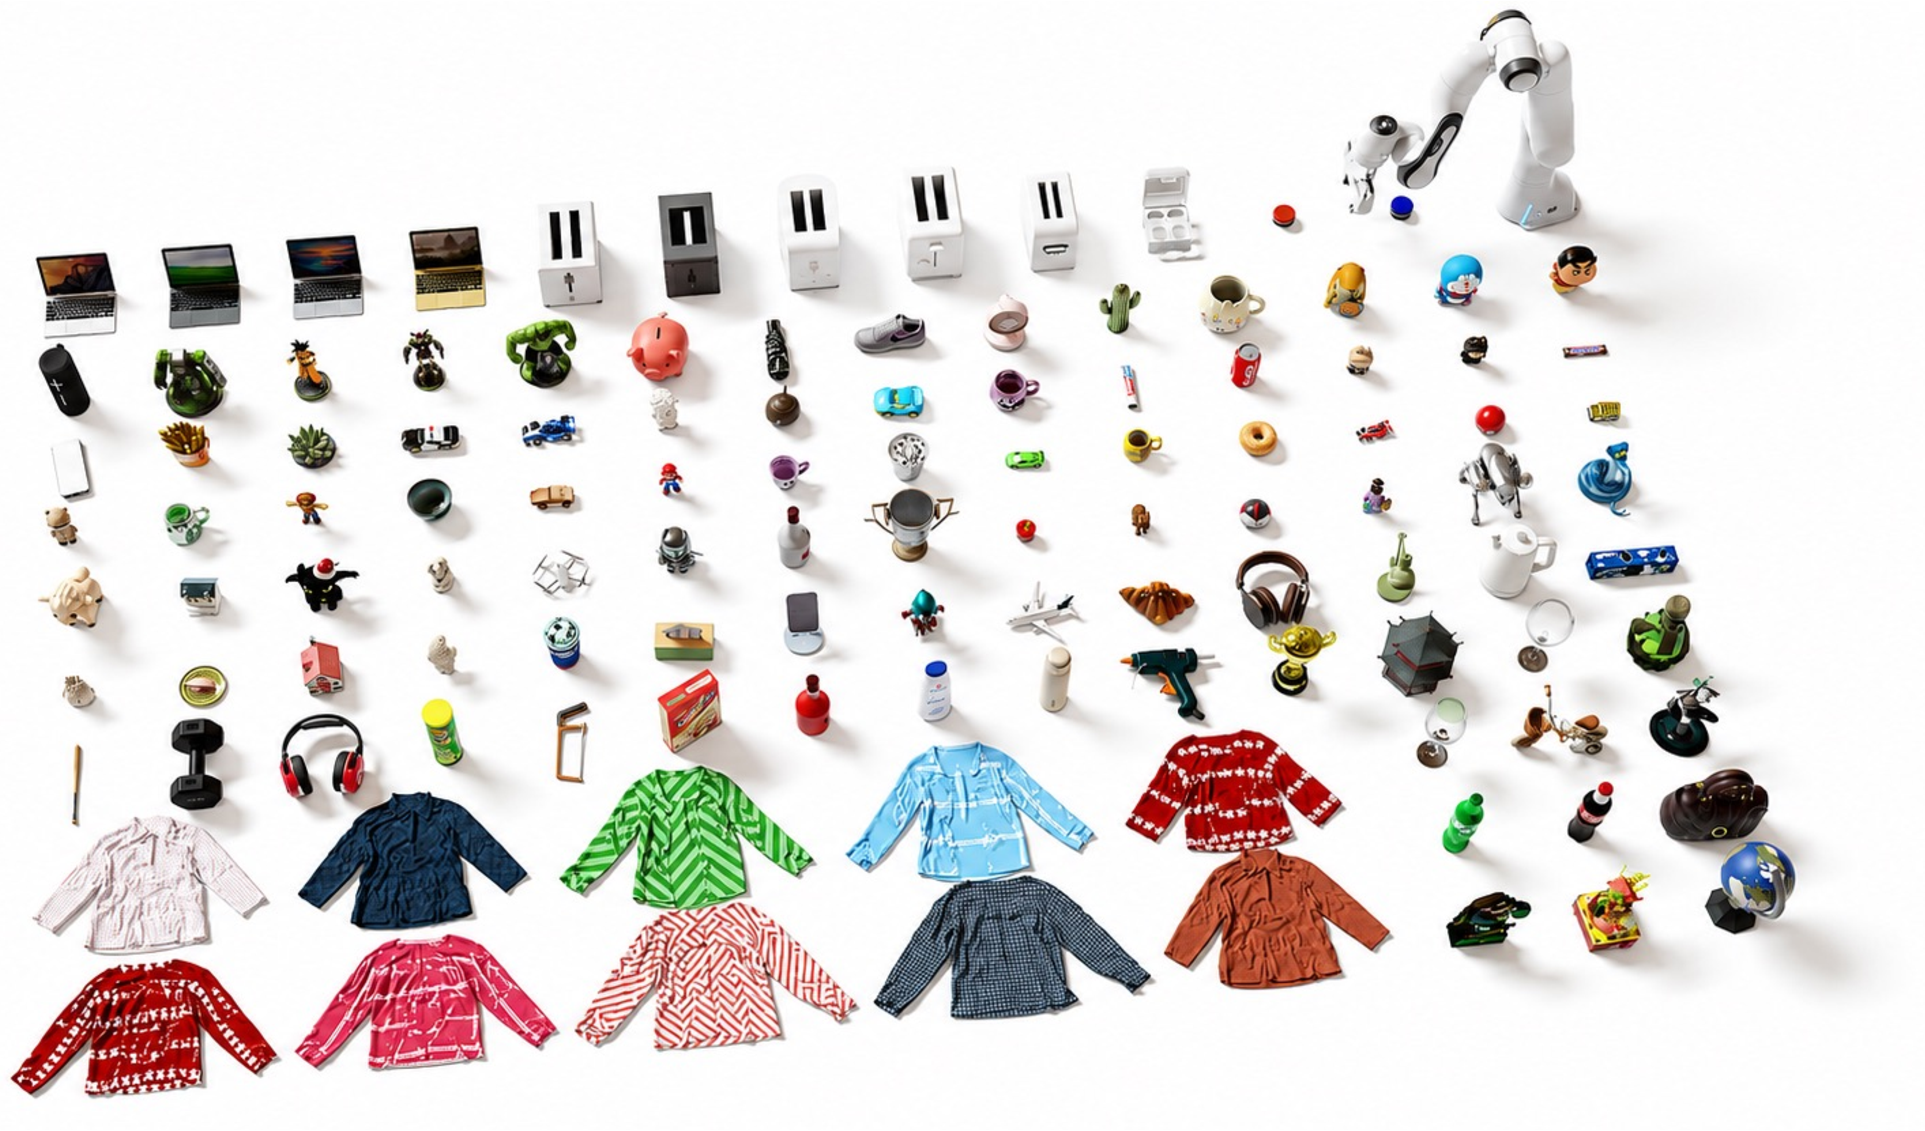
\includegraphics[width=\linewidth]{assets/Figure/assets.pdf}
        \caption{\textbf{Asset library.} Sample rigid, articulated, and deformable assets.}
        \label{fig:assets_library}
    \end{subfigure}
    \hfill
    \begin{subfigure}[t]{0.48\textwidth}
        \centering
        \roundedimage[6pt]{assets/Figure/parallel_scene.jpg}
        \caption{\textbf{Parallel simulation.} Concurrent heterogeneous task execution.}
        \label{fig:parallelism}
    \end{subfigure}
    \caption{\textbf{Assets and parallelism in RoboDojo.} RoboDojo combines physically grounded assets with heterogeneous parallel simulation for scalable benchmark construction and evaluation.}
    \label{fig:assets_parallelism}
\end{figure}

\subsubsection{Heterogeneous Parallelism}
\label{sec:parallelism}

Efficient benchmark evaluation requires parallel simulation over diverse scenes. Standard vectorized simulation often relies on homogeneous cloned environments, where parallel instances share the same scene template and differ mainly in poses or random seeds. While efficient, this setting is insufficient for evaluating generalist manipulation policies, which should be tested across diverse object geometries, object counts, clutter layouts, articulated structures, and background conditions.

RoboDojo therefore supports heterogeneous parallel simulation. Multiple environments are stepped under a shared vectorized interface, while each environment maintains an independently sampled scene configuration. Different parallel environments can contain different object categories, asset geometries, numbers of distractors, articulation structures, and task layouts. This design improves evaluation speed while preserving the scene-level diversity required for robust policy assessment. Implementation details of heterogeneous parallelism and multi-GPU sharding are provided in Appendix~\ref{appendix:heterogeneous_parallelism_details}.

\subsubsection{Simulation Data Collection}

RoboDojo supports two complementary data collection modes: automated trajectory synthesis and VR-based teleoperation. Both modes use a shared asset annotation layer that specifies manipulation-related affordances and task semantics, including graspable regions, placement regions, functional parts, and task-specific interaction points. These annotations support automated skill grounding and task validation.

For automated synthesis, RoboDojo composes demonstrations from reusable low-level skills, such as \texttt{grasp}, \texttt{place}, \texttt{handover}, \texttt{insert}, \texttt{open}, \texttt{close}, \texttt{stack}, and \texttt{push\_up}. Each skill is grounded in asset annotations and executed with the cuRobo v2 motion planner~\citep{sundaralingam2026curobov2dynamicsawaremotiongeneration}. For tasks that are difficult to synthesize automatically, RoboDojo provides a VR-based teleoperation interface for collecting high-quality demonstrations. Details on skill composition, motion planning, and teleoperation control are provided in Appendix~\ref{appendix:simulation_data_collection_details}.